%\addbibresource{/home/jorgsk/phdproject/bibtex/jorgsk.bib}

%What results should you present? Anything more than was presented in the paper?

%The figure with the compartments and poly(A)-.

%Shows two things: 1) there is poly(A) signal in poly(A)- extract. explained by
%errors in screening and possibly by short poly(A). 2) intronic polyadenylation in the nucleus overrepresented. Makes
%sense if there is nuclear degradation of intronic poly(A) which has been
%recently shown.

%Then the figure with overlap to show how much you get?

%Then the figure that shows the flattening out of the getting of new
%transcripts.

%Discuss each of the tree figures and that's it.

%Maybe make a table with some of the numbers from the statistics you output.

%Then cite the paper.
\subsection{Summary of the paper}
Summarize the paper.

\subsection{The dataset}
The datasets used in this study were generated by the ENCODE
(\textbf{Enc}yclopedia \textbf{O}f \textbf{D}NA \textbf{E}lements) consortium
and are available from http://hgdownload-test.cse.ucsc.edu/goldenPath/hg19/encodeDCC/wgEncodeCshlLongRnaSeq/

The data is from RNA-seq experiments from 12 human cell lines and their
nuclear and cytoplasmic compartments. Table \ref{tab:Datasets} shows the cell
lines and compartments used; as can be seen, most experiments were available
with a biological replicate. In total, 23 datasets were from whole cell
extracts, 11 were from cytoplasmic extracts, and 12 were from nuclear extracts.
For each cell line and compartment, datasets are available both for the
poly(A)+ and poly(A)- fraction of the RNA pool. This brings the total to 92
RNA-seq datasets. The RNA pool contains only long RNA, that is, RNA over 200
nucleotides in length. Each dataset has been generated with Illumina
paired-ended sequencing with a read-length of 75 basepairs. Each dataset
contains between 150 and 250 million reads.

\begin{table}
	\centering
	\begin{tabular}{cccc}
	  Cell line & Whole Cell & Cytoplasm & Nucleus \\
	  \midrule
	  GM12878 & 2 & 2 & 2 \\
	  K562 & 2 & 2 & 2 \\
	  HeLa-S3 & 2 & 2 & 2 \\
	  HUVEC & 2 & 2 & 2 \\
	  HEPG2 & 2 & 2 & 2 \\
	  H1Hesc & 1 & 1 & 1 \\
	  Nhek & 2 & 0 & 1 \\
	  MCF7 & 2 & 0 & 0 \\
	  AG04450 & 2 & 0 & 0 \\
	  HSMM & 2 & 0 & 0 \\
	  NHLF & 2 & 0 & 0 \\
	  A549 & 2 & 0 & 0 \\
	\end{tabular}
	\caption{Number of replicates of the datasets from the ENCODE consortium}
	\label{tab:Datasets}
\end{table}

What sets this library apart from most RNA-seq data is that the cell is
compartmentalized and that both the poly(A)+ and poly(A)- fractions of RNA have
been sequenced separately; these extra dimensions increase the resolution of
the data, allowing different hypotheseses to be asked. The poly(A)+ fraction of
an RNA sample contains all the RNA that is captured by a poly(T) primer column.
This will include all processes mRNA with a poly(A) tail of more than 20
nucleotides (the length of the poly(T) primer). The poly(A)- fraction is the
complement of the poly(A)+ fraction and contains mostly noncoding RNA and
pre-processed mRNA.

\subsection{The short RNA mapper}
The short read mapper used in this work is the GEM mapper
\cite{ribeca_gem_2010}. The GEM mapper is developed in the group of Roderic
Guigo and is production ready, although it has not been published yet.

\section{Results}
We developed a software called Utail and ran it on the ENCODE RNA-seq data.
For details on how Utail works, see the Appendix. Parts of the analysis from
Utail's output was published in XXX. The description of the methods we used are
found in the supplementary materials of the paper. Here we describe the parts
of the analysis which was not included in paper.

\subsection{Total number of polyadenylation sites}
By merging all polyadenylation sites from all poly(A)+ samples, a total of
108.000 polyadenylation sites were identified. Figure \ref{fig:saturation}
shows how the number of new polyadenylation sites saturates as the number of
datasets increases. The saturation is sharper for polyadenylation sites with a
downstream PAS, indicating that the number of false positives increases when
the number of reads becomes very large.

This is simply because each dataset has got falsely marked poly(A) sites, and
with each added dataset there is a chance that several of them will overlap the
same place.

\subsection{Distribution of polyadenylation sites across the genome}
We found that most of the polyadenylation sites are in the 3\p UTR exonic
regions, as expected, but there are also many polyadenylation sites in the
intergenic and intronic regions as well \ref{fig:sidebars}. The distribution of
polyadenylation sites varied between the whole cell and the cell compartments.
In general, the results from the whole cell extract is most similar to the
cytoplasmic extract, while the nuclear extract is most different, 
see Figure \ref{fig:sidebars}. The polyadenylation in intergenic regions
indicate either unannotated long 3\p UTR ends or cleavage and polyadenylation
sites of novel transcripts.

\subsection{Polyadenylation in the cell's poly(A)- fraction}
We also found evidece for polyadenylated RNA in the poly(A)- fraction, see
Figure \ref{fig:sidebars} B. This was unexpected, since the poly(A)- fraction
is supposed by design not to contain RNA with poly(A) tails. The polyadenylated
RNA in the poly(A)- fraction have three possible sources. Source one (S1) is
normal poly(A)+ mRNA with full length polyA tails that did not get absorbed by
the poly(A)+ filtration step and thus ended up in the poly(A)- fraction. Source
two (S2) is mRNA with polyA tails shorter than 20nt; either they have had
their polyA tails degraded to below 20 nucleotides, or they were actively
undergoing polyadenylation at the time of sampling and did not reach a poly(A)
tail length of more than 20 nucleotides. Source three (S3) are RNA with short,
degradation-related transient poly(A) tails. 

We wanted to separate the S3 from the S1 and S2 polyA sites. We did this by
recognizing that many of the S1 and S2 sites are likely to be present in both
the poly(A)- and the poly(A)+ fractions, since these sites really belong to
poly(A)+ transcripts that have accidentaly ended up in the poly(A)- fraction.
Therefore, we filtered out all the poly(A) sites that intersected the poly(A)+
and poly(A)- fraction and removed these from both fractions. As can be see in
in Figure \ref{fig:sidebars_intersect}, the difference between the cytoplasmic
and nuclear compartment increased when eliminating the poly(A) sites common to
both poly(A)+ and poly(A)-. The poly(A)- cytoplasmic fraction contains almost
no polyA sites, while the poly(A)- nuclear fraction remains enriched in polyA
sites, especially in the intronic region. The whole cell fraction is a
superposition of the nuclear and cytoplasmic fractions, as would be expected.

We believe that the enrichment of the poly(A)- polyA sites in the nuclear
fraction in general is due to degradation-related transient polyadenylation
that occurs in the nucleus of mammalian cells \cite{lemay_nuclear_2010,
lacava_rna_2005, wyers_cryptic_2005}. In the nuclear compartment, the intronic
region stands out, but part of this is due to the fact that introns comprise a
large part of nuclear RNA, since human pre-mRNA sequences contain over 20 times
more intronic than exonic sequence \cite{venter_sequence_2001}.

\begin{figure}[htb]
	\begin{center}
		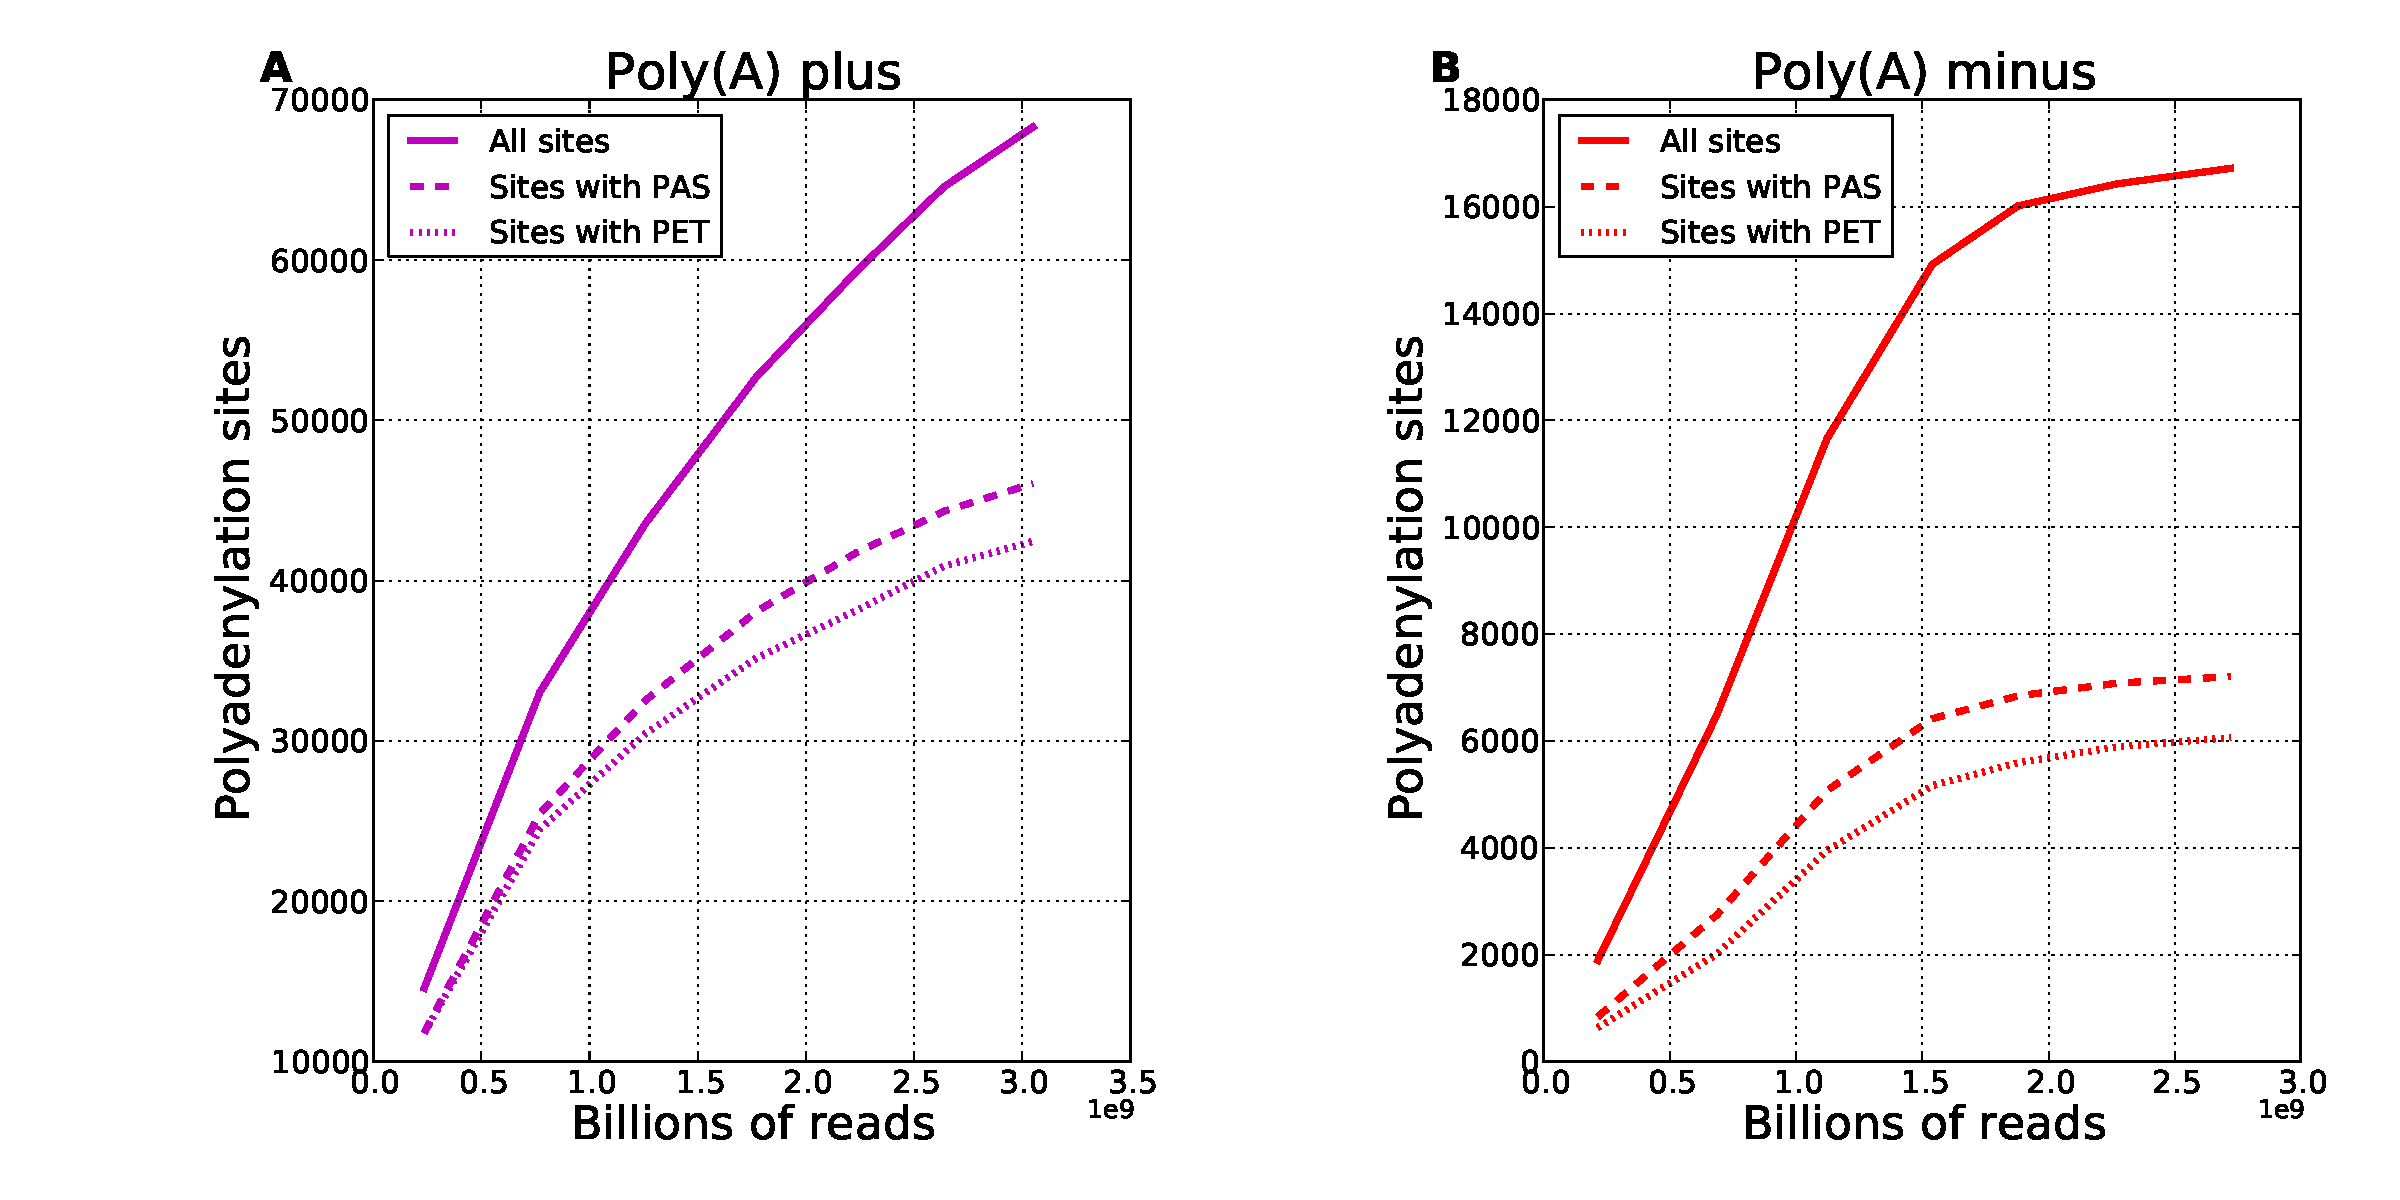
\includegraphics[scale=0.3]{figures/polyadenylation/Saturation_plot_2+.pdf}
	\end{center}
	\caption{Saturation of discovery of polyadenylation sites}
	\label{fig:saturation}
\end{figure}

\begin{figure}[htb]
	\begin{center}
		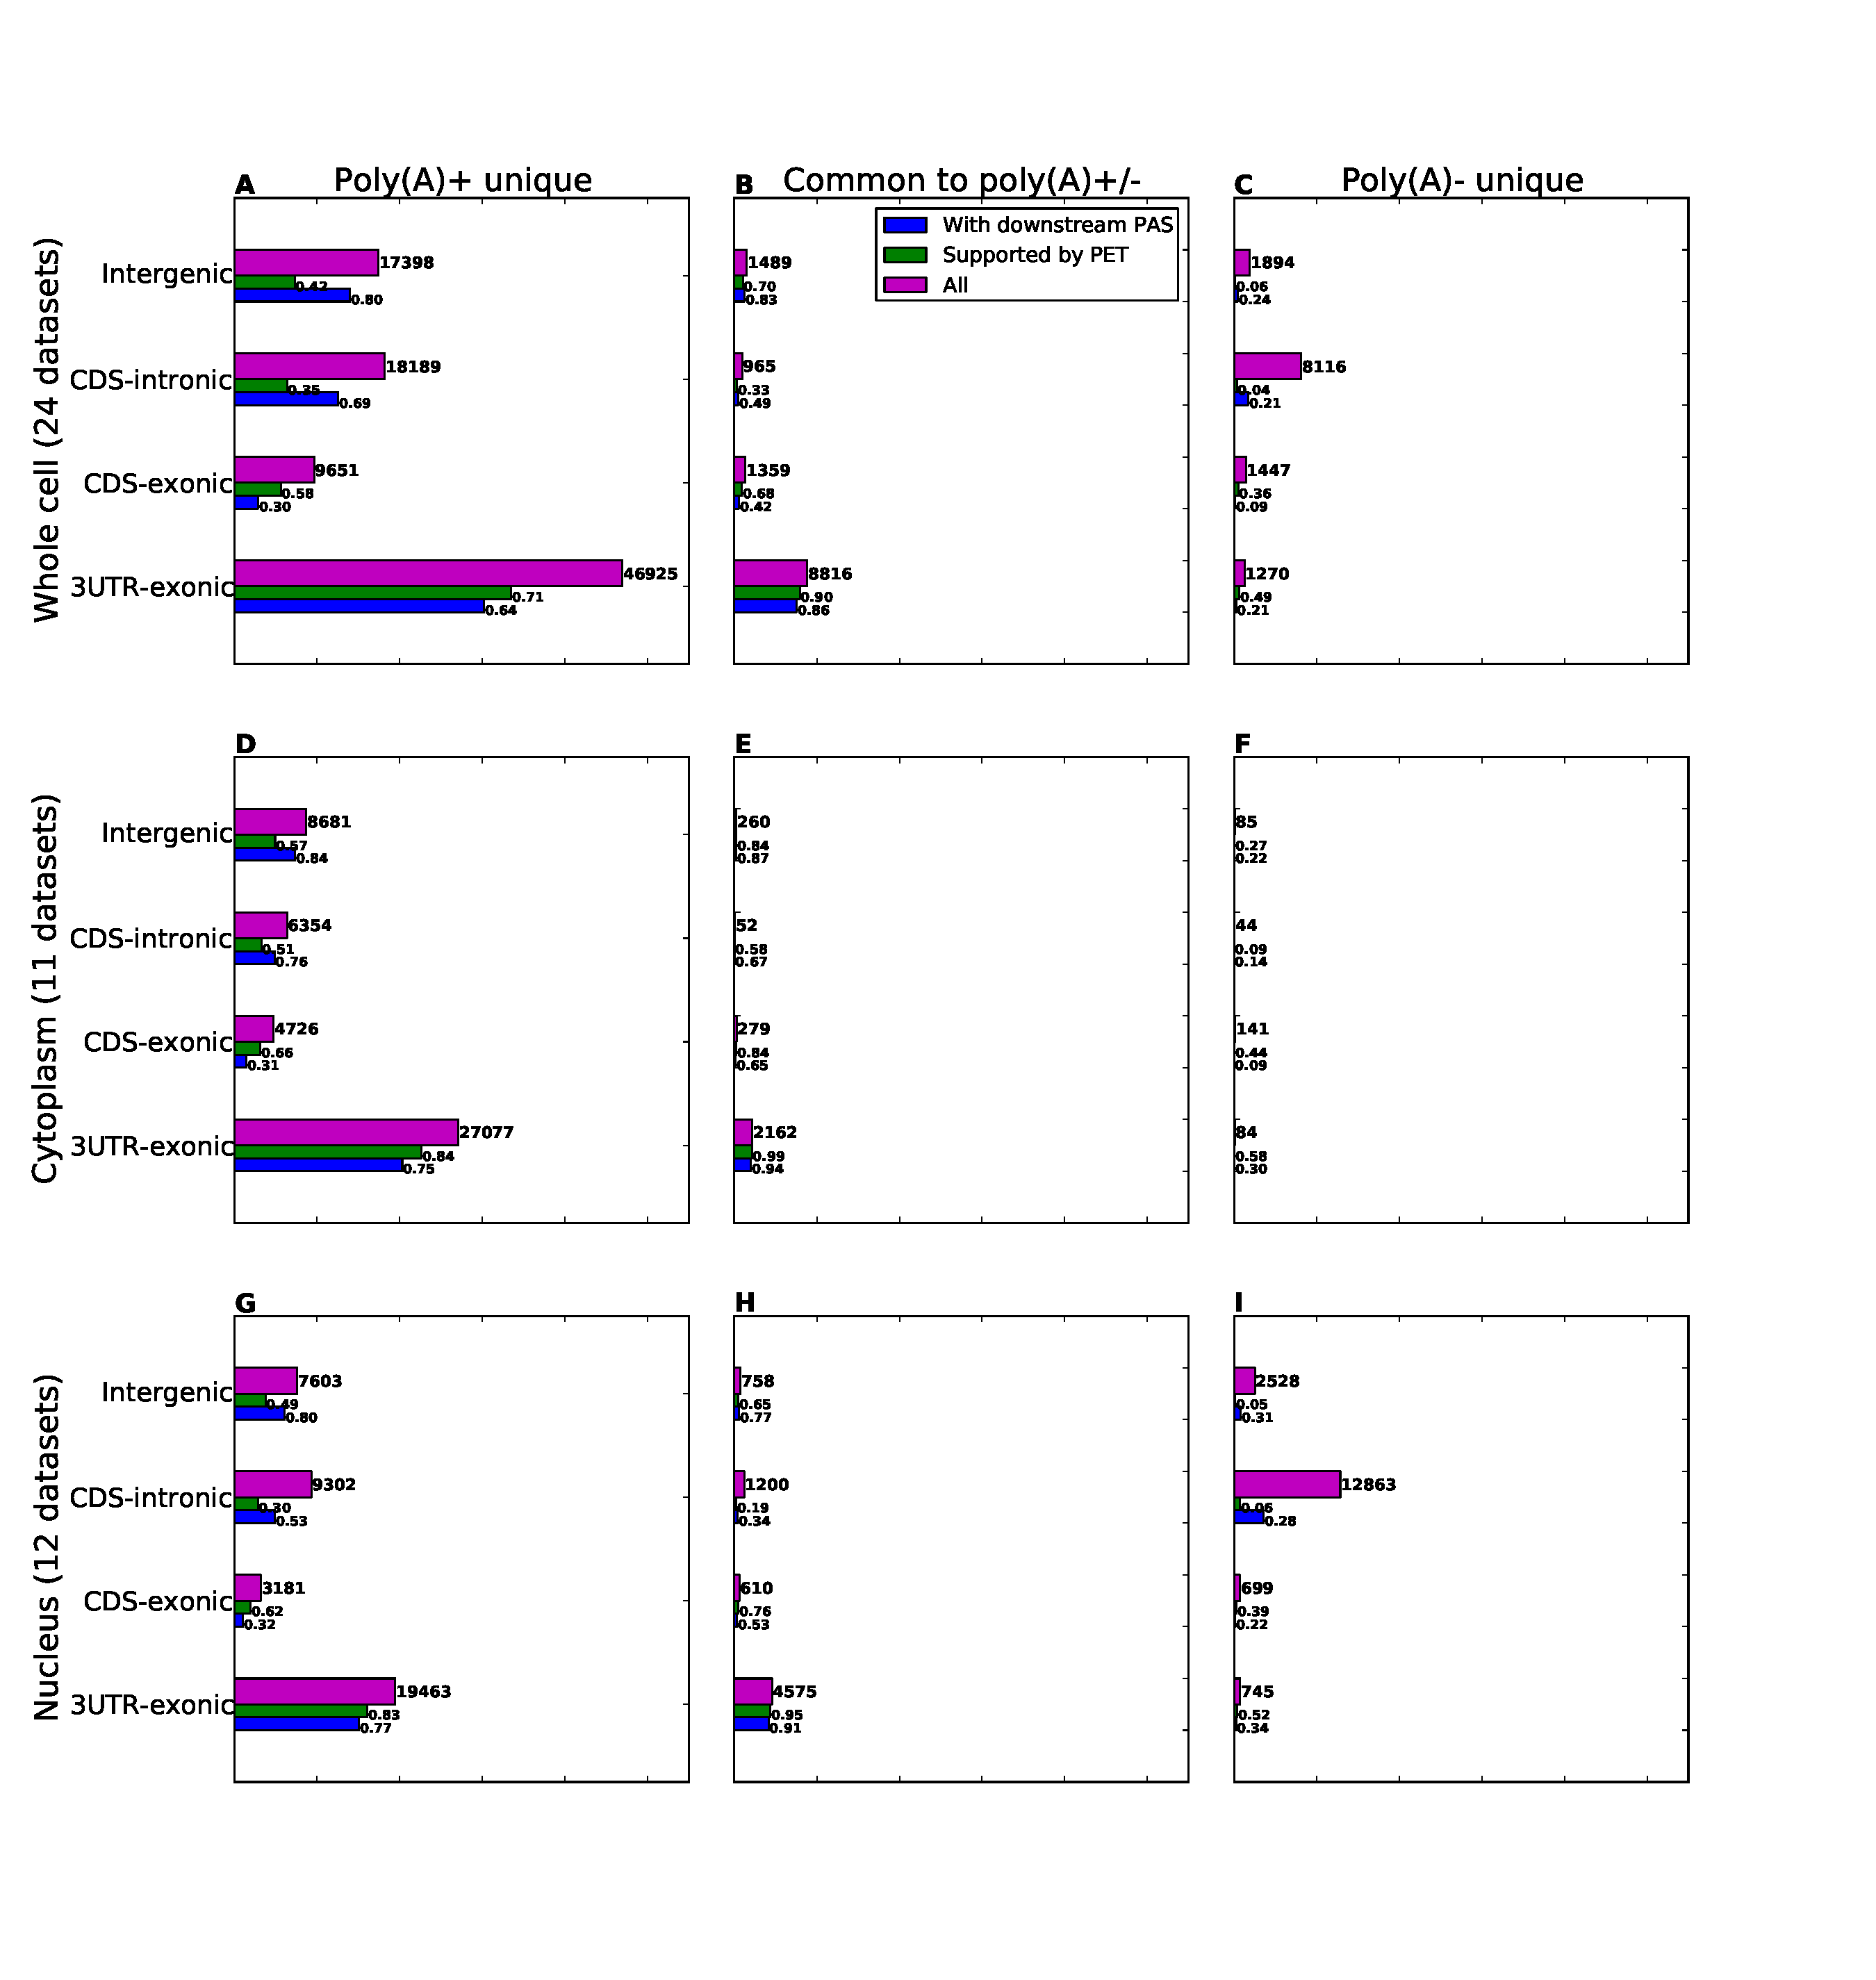
\includegraphics[scale=0.3]{figures/polyadenylation/intersected_sidebars_pA_2+.pdf}
	\end{center}
	\caption{Polyadenylation across genomic regions for the poly(A)+ and poly(A)-
	fractions and the sites that overlap the poly(A)+ and poly(A)- fractions}
	\label{fig:sidebars_intersect}
\end{figure}

\begin{figure}[htb]
	\begin{center}
		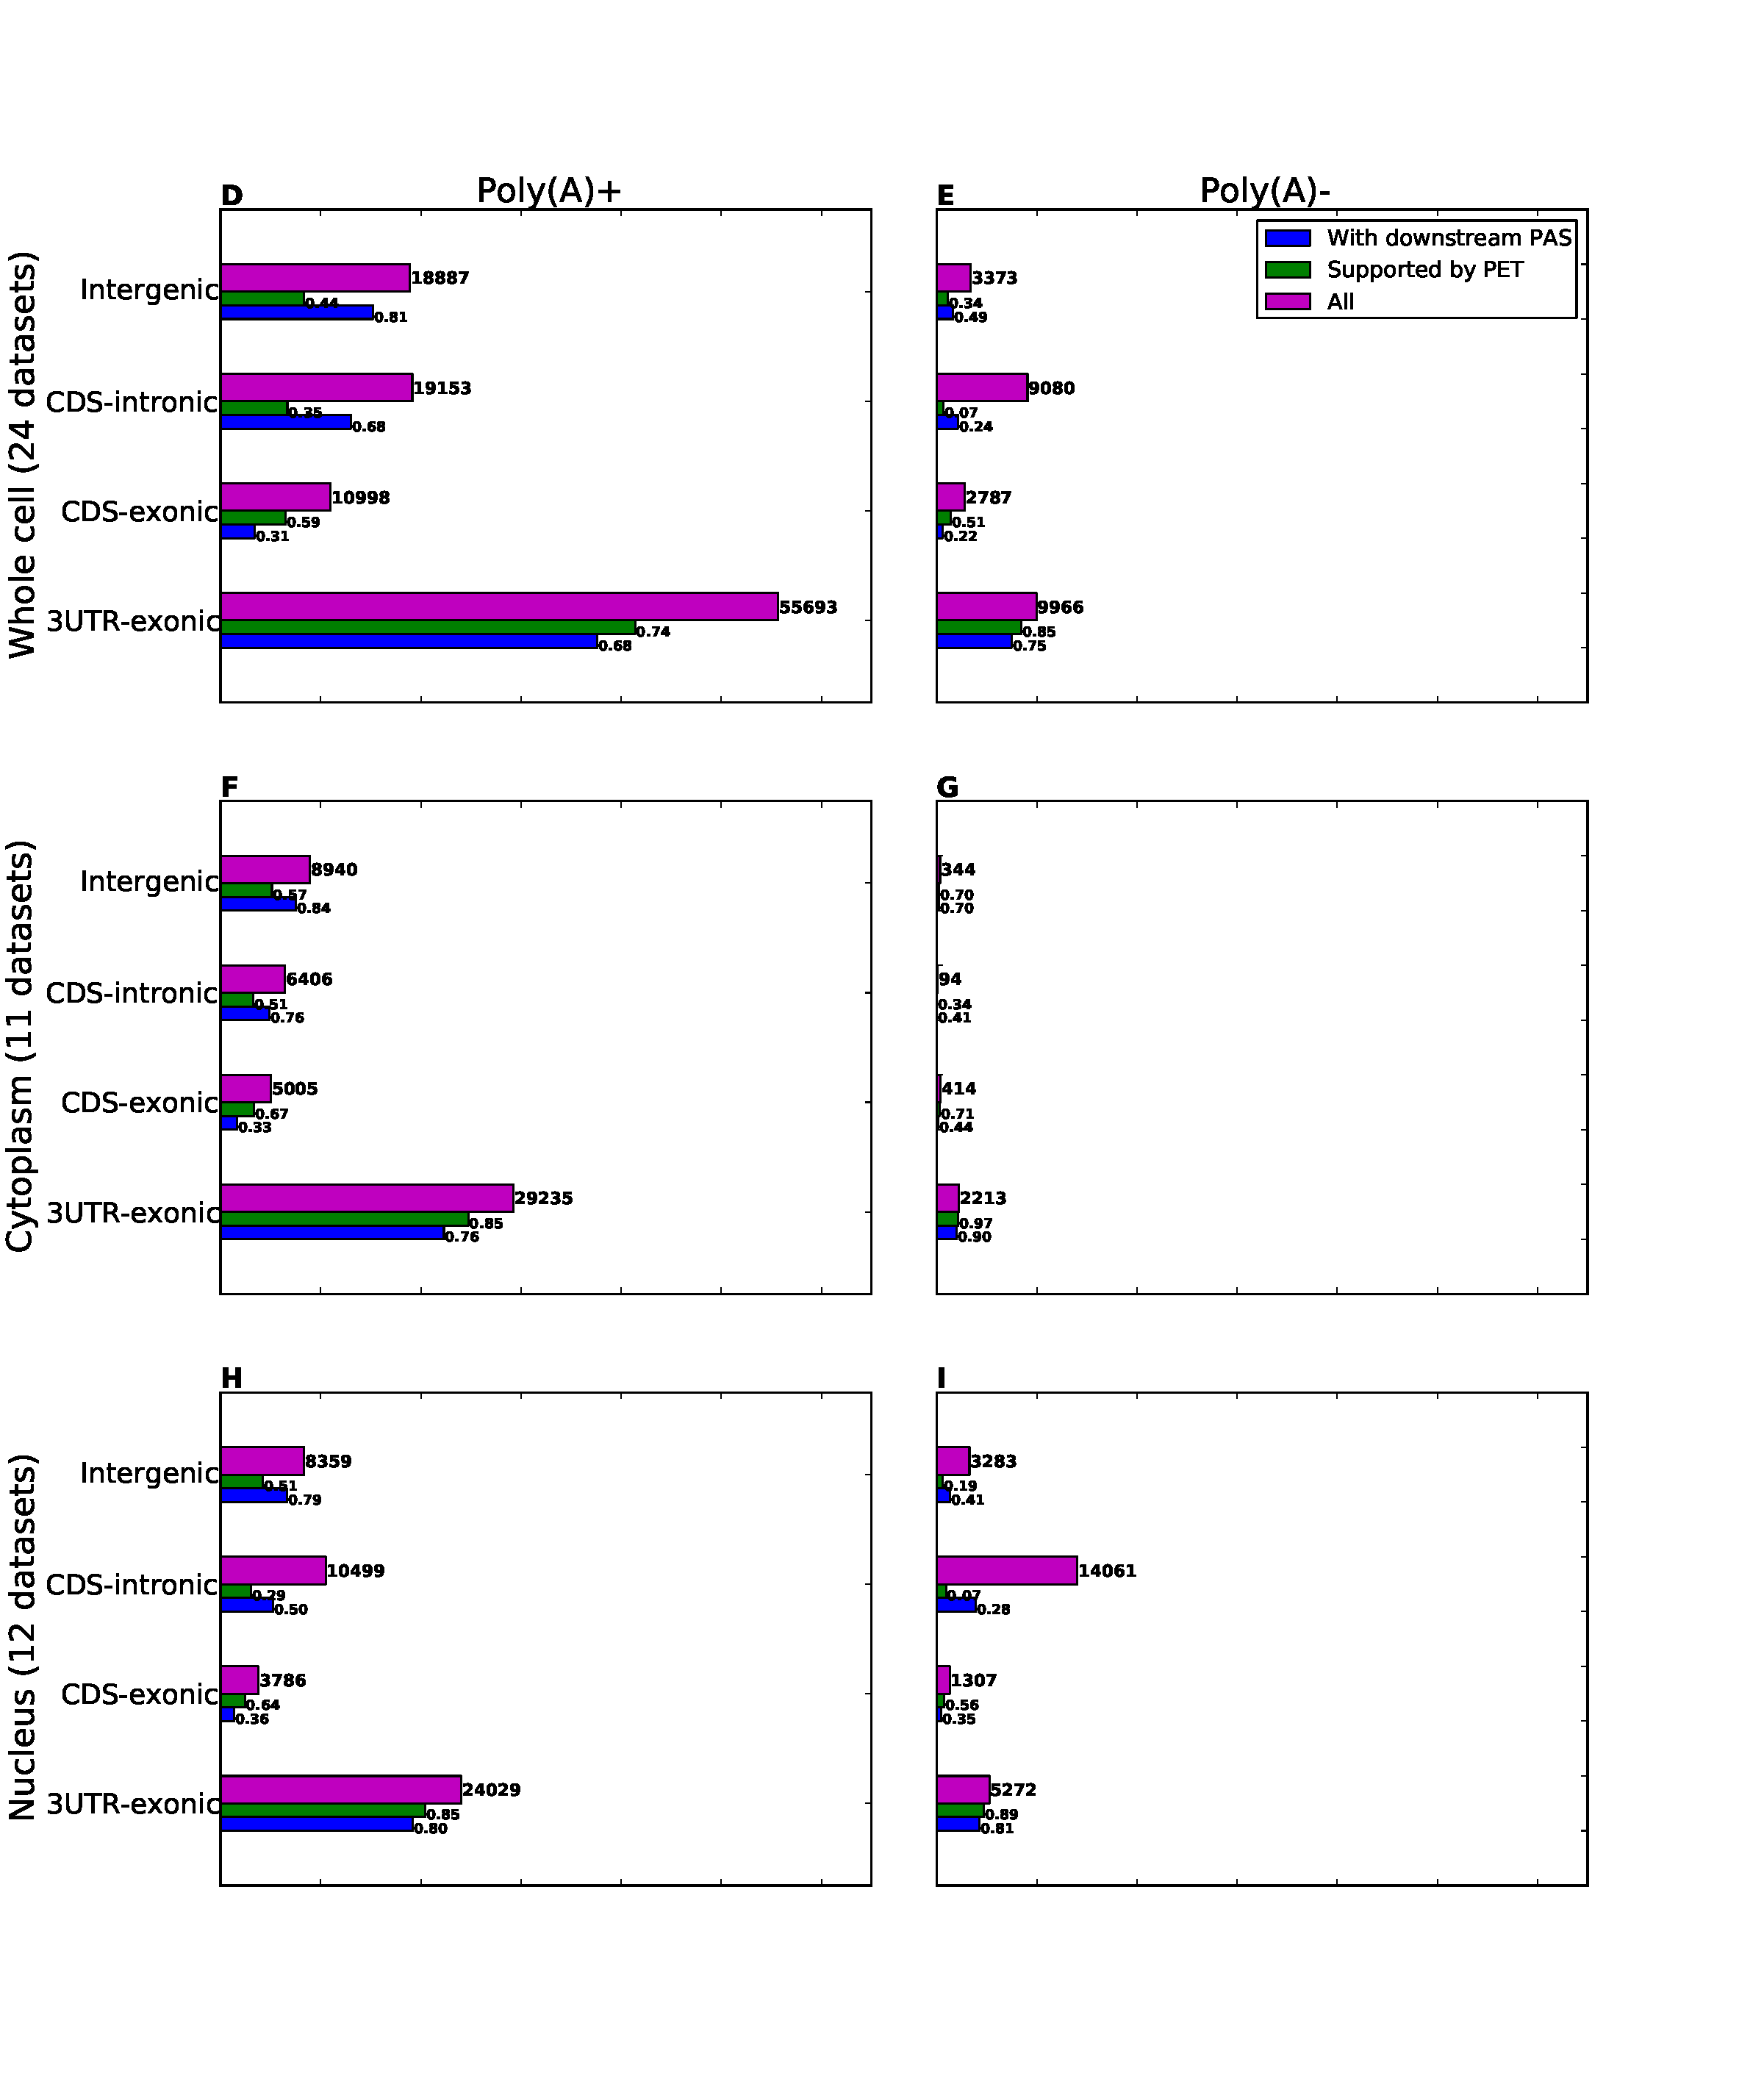
\includegraphics[scale=0.4]{figures/polyadenylation/Sidebars_pA_2+.pdf}
	\end{center}
	\caption{Polyadenylation across genomic regions for the poly(A)+ and poly(A)-
	fractions}
	\label{fig:sidebars}
\end{figure}

\subsubsection{Discussion}
